On the real-world datasets, we compare \method{} with the XGBoost black box, two GAMs (NAM and EBM) and two \gamms{}: EB$^2$M (EBM with pairwise interactions) and NODE-GA$^2$M.
We report accuracy for classification and RMSE for regression, and count a win or a loss only when two means differ by more than the larger of their standard deviations over the folds, a draw otherwise.
Figure~\ref{fig:dumbbell} shows what each model gains over the GAM on every dataset, and Tables~\ref{tab:clf-acc} and~\ref{tab:regr-rmse} (Appendix~\ref{app:main-tables}) give every baseline with its spread, including GAMI-Net.
\begin{figure}[t]
  \centering
  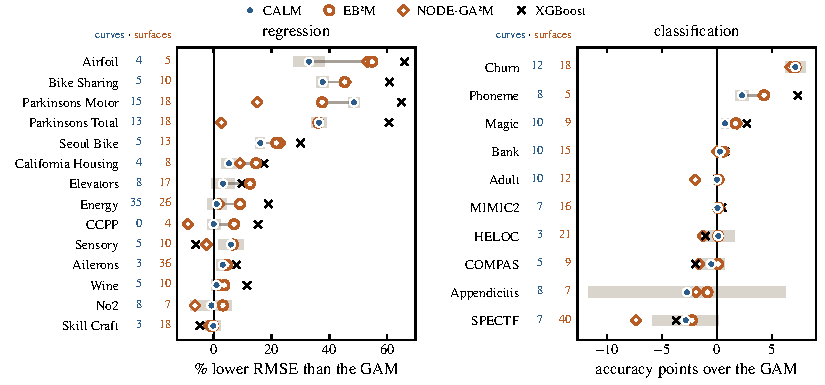
\includegraphics[width=\linewidth]{images/dumbbell}
  \caption{What each model gains over the GAM on each dataset: the black box XGBoost, the \gamms{} NODE-GA$^2$M and EB$^2$M, and \method{} (means over 5 folds, higher is better).
    The gray band behind each dot is $\pm\max(\mathrm{std}_{\text{\method{}}}, \mathrm{std}_{\text{EB}^2\text{M}})$ over the folds.
    A ring inside it is a draw, outside a win or a loss.
    \method{} ahead/level/behind:
    against the GAM, 8/6/0 in regression and 3/7/0 in classification;
    against EB$^2$M, 1/5/8 and 0/7/3 (see Tables~\ref{tab:clf-acc} and~\ref{tab:regr-rmse} for full results).
    Left of each row: the curves that \method{} adds on top of the GAM, and the pairwise surfaces that EB$^2$M fits.}
  \label{fig:dumbbell}
\end{figure}


\textbf{Classification results.}
On the 10 classification datasets (Fig.~\ref{fig:dumbbell}, right; Table~\ref{tab:clf-acc}), \method{}
(i) matches or beats each GAM on all datasets, tying with NAM on 5 and EBM on 7;
(ii) matches or beats each \gamm{} on most datasets, losing to EB$^2$M on 3 and to NODE-GA$^2$M on 2; and
(iii) matches or beats XGBoost on 6, losing on 4.

\textbf{Regression results.}
On the 14 regression datasets (Fig.~\ref{fig:dumbbell}, left; Table~\ref{tab:regr-rmse}), \method{}
(i) matches or beats each GAM on all datasets, tying with NAM on 4 and EBM on 6;
(ii) matches or beats NODE-GA$^2$M on 10, but loses to EB$^2$M on 8; and
(iii) matches or beats XGBoost on 3, losing on 11.

\textbf{Summary.}
In both tasks, \method{} improves over GAMs, closing the GAM-to-XGBoost gap by a median of 37\,\% in regression and of 31\,\% in classification.
Against the \gamms{}, it is competitive on most datasets, but it still trails: in regression, EB$^2$M is more accurate on 8 of the 14 datasets, on 7 of them by more than 5 points in Figure~\ref{fig:dumbbell}.
We attribute this gap, like the one to XGBoost, to \method{}'s stricter constraint: one-dimensional curves instead of two-dimensional surfaces.

\textbf{Complexity.}\label{sec:complexity}
We measure the complexity of a \method{} in two quantities: (i) the conditional interactions of Section~\ref{subsec:model-overview}, the features $x_j$ that are part of the partition tree $T_i$ of $x_i$ (Appendix~\ref{app:interactions}) and (ii) the number of curves it adds to the GAM, which we compare with a \gamm{}'s pairs and surfaces.
For (i), \method{} uses 6.6 conditional interactions on average in regression and 6.8 in classification (Tables~\ref{tab:classification_interactions} and~\ref{tab:regression_interactions}); for (ii), it adds 8.2 and 7.9 curves (Fig.~\ref{fig:dumbbell}, left of each row).
EB$^2$M fits 14.3 and 15.2 pairs, one surface each.
These numbers come from \method{}'s default configuration, which puts no cap on the number of interactions.
\method{} still finds a sparse structure, because a tree grows only when a split reduces heterogeneity enough (Step~1(b)), and the selection keeps only the trees that add fidelity to the reference model, i.e., that increase $R^2(\mathcal{S})$ (Step~1(c)).
This is a key advantage of \method{}: it adds an interaction only when the data asks for it.

\textbf{Sensitivity to hyperparameters.}
We vary $d_{\max}$ and $\gamma$ and find that only the depth affects accuracy and complexity substantially.
Over the datasets where XGBoost beats the GAM, i.e., where there is room for improvement (12 of 14 in regression, 5 of 10 in classification), the median share of that gap that \method{} closes grows from 17\,\% at $d_{\max}=1$ to 37\,\% at $d_{\max}=2$ and 49\,\% at $d_{\max}=3$ in regression (17, 31 and 41\,\% in classification), while the median number of conditional interactions roughly doubles per level (1.9, 4.5 and 9.6 in regression).
On Bike Sharing, deeper trees keep paying: $d_{\max}=6$ closes 85\,\% of the gap, against 62\,\% at the default depth, with 9.8 conditional interactions instead of 4.6 (Appendix~\ref{app:depth-ladder}).
In general, depth is a knob to trade interpretability for accuracy, and the default $d_{\max}=2$ is a good compromise.
Halving or doubling $\gamma$ changes the accuracy beyond one standard deviation on at most two of the 24 datasets, so its default is a safe choice.

\textbf{Runtime.}
On a laptop CPU (10 threads), \method{} fits 19 of the 24 datasets in under a minute (median 21\,s, at most 2\,min, on Energy), against a median of 4\,s for EBM on the same runs.
Most of this time is spent proposing the trees (Step~1(b), $\mathcal{O}(d_{\max}\, d^2 N \log N)$) and fitting the shape functions (Step~2).
NODE-GA$^2$M, timed earlier on other hardware, takes 1 to 2 minutes per fit (Tables~\ref{tab:clf-time-def}--\ref{tab:regr-time-def}).

\subsection{Stability}\label{sec:stability}
\begin{wraptable}{r}{0.47\textwidth}
\vspace{-1.2em}
\centering
\small
\setlength{\tabcolsep}{4pt}
\begin{tabular}{lcccc}
\toprule
& \multicolumn{2}{c}{folds} & \multicolumn{2}{c}{bootstrap} \\
\cmidrule(lr){2-3}\cmidrule(lr){4-5}
agreement on the & 5/5 & $\geq$4/5 & 5/5 & $\geq$4/5 \\
\midrule
interaction verdict & 77\,\% & 90\,\% & 74\,\% & 89\,\% \\
root conditioner & 74\,\% & 87\,\% & 71\,\% & 86\,\% \\
full structure & 71\,\% & 81\,\% & 68\,\% & 80\,\% \\
\bottomrule
\end{tabular}
\caption{Share of the 376 features on which the refits of \method{} agree.}
\label{tab:stability}
\vspace{-1em}
\end{wraptable}
We assess the stability of \method{}: does refitting it return similar trees?
This matters when \method{} is used not only to predict with an interpretable-by-design model, but also to learn about the process that generated the data.
We therefore refit \method{} on the 5 cross-validation folds (each on 80\,\% of the rows) and on 20 bootstrap resamples, and ask three questions of increasing strictness: (i) is the feature split at all (the \emph{interaction verdict}), (ii) on which feature is its root split (the \emph{root conditioner}), and (iii) is its whole tree the same (the root and the depth-2 conditioners, the \emph{full structure}); ``not split'' counts as an answer.
Each question is asked separately of each of the 376 features of the 24 datasets.
Table~\ref{tab:stability} gives the share of features on which all 5 refits agree, or at least 4; the bootstrap shares are averaged over 4 disjoint groups of 5 resamples.
On whether a feature is split, 77\,\% of the features agree across all five folds and 90\,\% across four; agreement falls only a few points as the question becomes stricter, to 71\,\% and 81\,\% for the full structure, and the bootstrap, which perturbs the data more, lowers each share by one to three points.
Where a rule recurs, its threshold barely moves: over the 88 rules found in at least 3 of the 5 folds, the median spread of the threshold is 0.08 standard deviations of the feature, and 73\,\% stay within 0.2.

\subsection{User study}\label{sec:user-study}
In an online study, 25 participants, from novices to experts in machine learning (13 self-reported advanced or expert), answered questions on the effect of the hour in a Bike Sharing model, once from \method{}'s conditional curves and once from a \gamm{}'s main effect and heatmaps: how the prediction changes when the hour moves.
Participants answered 54\,\% of the questions correctly with \method{} and 34\,\% with the \gamm{} ($p<0.05$), and the gap is widest on the question of how long the hour takes to lower the prediction (40\,\% vs.\ 12\,\%).
The advantage holds among the 13 advanced or expert participants, for whom heatmaps are standard tooling (65.4\,\% vs.\ 30.8\,\%, Wilcoxon $p=0.031$), and accuracy with the \gamm{} does not rise with expertise (Spearman $\rho=-0.29$, $p=0.14$); Appendix~\ref{app:user-study} gives the design, the questions and the grading.
